\documentclass[conference]{IEEEtran}
\IEEEoverridecommandlockouts
\usepackage{amsmath,amssymb,amsfonts}
\usepackage{algorithmic}
\usepackage{graphicx}
\usepackage{textcomp}
\usepackage{xcolor}
\usepackage{float}
\usepackage{dblfloatfix}
\usepackage[sorting=none, style=nature]{biblatex}
\addbibresource{ref.bib}
\usepackage[hidelinks]{hyperref}


\def\BibTeX{{\rm B\kern-.05em{\sc i\kern-.025em b}\kern-.08em
T\kern-.1667em\lower.7ex\hbox{E}\kern-.125emX}}
\begin{document}

    \title{Public Ledger for Auctions}

    \author{\IEEEauthorblockN{Cláudia da Costa Maia}
    \IEEEauthorblockA{up201905492@fc.up.pt}
    \and
    \IEEEauthorblockN{Fabiana Manuela Alves}
    \IEEEauthorblockA{up201404791@fc.up.pt }
    \and
    \IEEEauthorblockN{Junior Monteiro}
    \IEEEauthorblockA{up202209374@fc.up.pt}
    }

    \maketitle
    \begin{abstract}
        Este projeto tem como objetivo criar uma rede \textit{Kademlia} com blockchain para uma aplicação de leilões descentralizada e segura. A rede \textit{Kademlia} será responsável por gerenciar participantes e leilões, enquanto a blockchain armazenará todas as ofertas e transações realizadas. A implementação inclui conceitos de P2P e DHT, mecanismos de criptografia e autenticação. O algoritmo de Proof-of-Work é utilizado para validar as transações e adicionar novos blocos à blockchain.

    \end{abstract}


    \begin{IEEEkeywords}
        Secure P2P; Kademlia DHT; Sybil and Eclipse attacks; Auction mechanisms; Distributed ledger; Blockchain; Blocks; Proof-of-Work; Proof-of-Stake; BFT
    \end{IEEEkeywords}


    \section{Introdução}
    Neste projeto utilizamos uma blockchain pública e os nós comunicam entre eles usando um protocolo de rede peer-to-peer (P2P), a \textit{Kademlia}, podendo descobrir outros nós na rede por meio de mecanismos de descoberta, implementados na \textit{Kademlia}. A blockchain é baseada numa abordagem sem permissão, ou seja, pública, já que qualquer pessoa pode participar na rede como um nó (enviar transações e validar blocos), logo não há uma entidade centralizada que controle quem pode participar. Isso significa que os nós não precisam de ser conhecidos à priori, ou seja, não é necessário um convite ou permissão para entrar na rede.
    O projeto foi dividido em três partes: (1) sobreposição P2P segura (\textit{Kademlia}), (2) registro distribuído e seguro (Blockchain) e (3) mecanismos de leilão (Aplicação).\\


    \section{Sobreposição P2P segura (\textit{Secure P2P overlay})}

    A sobreposição P2P é baseada em \textit{Kademlia} DHT e é responsável por gerenciar os nós participantes da rede. Para garantir a segurança da rede, são implementados mecanismos de confiança e de comunicação gossip.

    \subsection{Kademlia DHT}
    O protocolo \textit{Kademlia} é um sistema de tabela de hash distribuída (DHT) usado para localizar nós na rede P2P e armazenar informações de forma descentralizada.

    O \textit{Kademlia} é baseado numa chave de 160 bits, que é usada para identificar cada nó na rede e usa a distância (XOR entre os IDs) para medir a proximidade entre os nós e organizar a rede num espaço métrico. Cada nó contém: \textit{node, routing\_table, store\_values, service, bt}. Sendo que o \textit{node} contém \textit{id, ip e port}. O atributo \textit{bt} refere-se ao \textit{bootstrap node} a que cada nó comum está associado.

    Os nós mantêm informações sobre os outros nós numa tabela, \textit{Routing table}, dividida em \textit{k-buckets} de acordo com a proximidade das chaves. A estrutura que usamos para a \textit{Routing table} foi uma tabela hash que armazena por ordem os \textit{k-buckets} em função da proximidade ao nó (dos nós mais proximos aos nós mais distantes). Desta forma, a \textit{Routing table} reflete a topologia da rede, armazenando nós vizinhos próximos e excluindo nós distantes e é dinamicamente atualizada à medida que o nó interage com a rede.
    Através da \textit{Routing table}, um nó na rede Kademlia pode determinar quais os nós que estão mais próximos de um determinado ID, permitindo o encaminhamento eficiente de mensagens e a busca rápida de nós responsáveis por determinadas chaves de dados. A \textit{Routing table} desempenha um papel fundamental na escalabilidade e eficiência da rede Kademlia.

    Cada \textit{k-bucket} contém informações sobre até k nós mais próximos a uma determinada chave. Estas informações sobre os respetivos nós são: \textit{ip, port e id}.
    Assim, se a \textit{Routing table} de um nó já tiver o número máximo de nós num determinado \textit{k-bucket}, ele remove o nó mais antigo nesse \textit{k-bucket} para libertar espaço para o novo nó. Para além disso, um nó é também eliminado do \textit{k-bucket} se nunca responder, ou seja, se o seu grau de confianca for muito baixo.

    Dentro da rede existem nós comuns, que fazem parte da rede e são responsáveis por armazenar e encaminhar os dados. E, nós \textit{bootstrap}, de inicialização, que conhecem todos os outros nós e são os nós responsáveis por ajudar os novos nós a integrarem-se na rede. Esses nós são pré-configurados e conhecidos pelos desenvolvedores da rede. Quando um novo nó entra na rede, ele contacta primeiro um ou mais nós de inicialização para obter informações sobre a topologia da rede.

    \textit{Inter-Node Messaging} é a comunicação feita entre os nós, e no protocolo \textit{Kademlia} são usados quatro tipos de chamadas de procedimento remoto (RPCs) para permitir esta comunicação:

%%%%%%%%%meti aqui a imagem para aparecer na pagina anterior........
    \begin{figure*}[b]
        \centering
        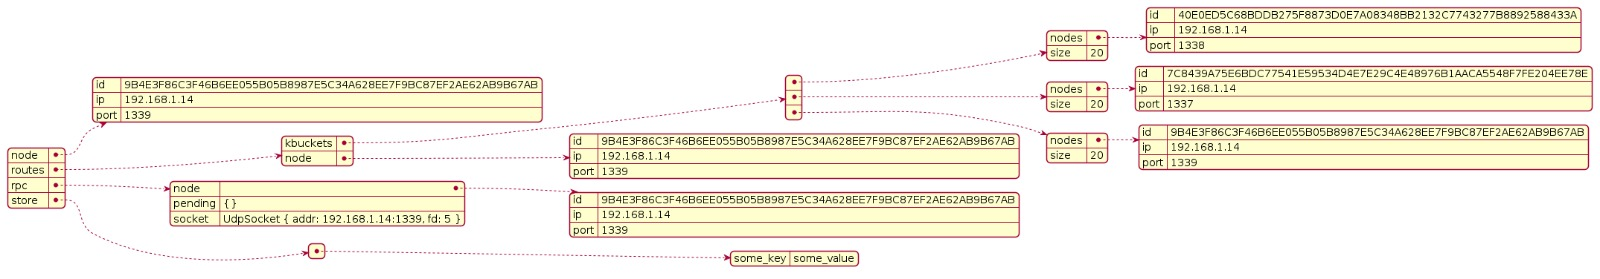
\includegraphics[width=\textwidth]{images/kademlia-estrutura.jpeg}
        \caption{Estrutura Kademlia \cite{1}}
        \label{fig:Estrutura Kademlia}
    \end{figure*}
%%%%%%%%%

    \begin{itemize}
        \item \textbf{ping:} é usado para verificar se um nó está online ou não. Quando um nó recebe uma mensagem Rpc::Ping, este responde com uma mensagem Rpc::Pong para o remetente.
        \item \textbf{store:} é usado para instruir um nó a armazenar um par de chave-valor no seu armazenamento local. Para isto, é fornecido a esta função a chave e o valor, assim como o nó destino onde vai ser guardada a informação. O nó emissor começa por procurar o nó responsável por essa chave na sua tabela de roteamento. Caso o nó responsável não esteja presente na tabela de roteamento, é feita uma busca pela rede para encontrar os nós mais próximos ao ID da chave. Após encontrar o nó responsável pela chave ou os nós mais próximos, o nó emissor envia uma mensagem Rpc::Store contendo a chave e o valor para o nó destino. A mensagem Rpc::Store é transmitida de forma direta entre o nó emissor e o nó destino, sendo que o nó destino é adicionado à routing table do nó emissor e vice-versa. Quando o nó destino recebe a mensagem \textit{store}, este armazena o valor em \textit{store\_values}.
        Após armazenar o valor, o nó destino envia uma resposta de confirmação, um Rpc::Pong, para o nó emissor indicando que o armazenamento foi concluído com sucesso. Caso contrario, o \textit{store} não é efetuado.

        \item \textbf{find\_node:} é usado para obter informações sobre os k nós mais próximos de um determinado ID de destino. O destinatário da mensagem responde com \textit{FindNodeReply} e fornece uma lista dos k nós mais próximos que tem na sua \textit{Routing table}. De seguida, o nó emissor atualiza a sua \textit{Routing table} com estes nós que lhe foram fornecidos.

        \item \textbf{find\_value:} Esta mensagem Rpc::FindValue é semelhante a \textit{Rpc::FindNode}, mas se o destinatário da mensagem já tiver o nó com o valor pedido na sua \textit{Routing table}, em vez de o \textit{Rpc::FindNodeReply} retornar a lista dos nós mais próximos, retorna o próprio nó com o valor pedido.
    \end{itemize}
    Estes RPCs são usados pelos nós para interagir uns com os outros e para executar várias operações, como armazenar e recuperar dados, bem como manter a topologia da rede.

    Para além disso, para que um nó entre na rede temos a função \textit{bootstrapping}. Neste caso, o nó em inicialização envia uma requisição de \textit{bootstrapping} para um ou mais nós conhecidos na rede. O objetivo é obter informações sobre a topologia da rede e construir sua \textit{Routing table} inicial. Assim, para este processo o nó começa por calcular o seu ID na rede kademlia usando a função de hash sha-1 e o seu IP e Porta (sendo que o IP e Porta deste novo nó é configurado à priori manualmente). Após calcular o ID o nó seleciona um ou mais nós bootstrap para enviar a requisição \textit{bootstrapping} com o seu ID, IP e Porta. Assim, o nó dá-se a conhecer à rede e é registado nas \textit{Routing tables} dos outros nós, e constrói através da função \textit{boostrappingReply} a sua propria \textit{Routing table}.
    É de notar que para o nó se conseguir juntar à rede tem de conseguir resolver o desafio de criar o seu ID com 4 zeros no inicio através de várias iterações da função de hash. Isto é feito para prevenir que se juntem à rede nós para apenas a saturar.

    Com a figura \cite{1} podemos ter uma melhor ideia como está estruturado cada nó da rede, assim como os seus atributos.

    \subsection{Mecanismos de confiança e de comunicação gossip}
    Os mecanismos de confiança são métodos utilizados para avaliar a credibilidade e a confiabilidade dos participantes num sistema distribuído. Permitem que nós (ou usuários) determinem a confiabilidade de outros nós na rede com base nas suas interações passadas. Esses mecanismos ajudam a prevenir atividades maliciosas, como ataques de \textit{Sybil} ou fraudes.
    Neste projeto são utilizados mecanismos de confiança baseados em reputação de nós, onde os nós acumulam uma pontuação de reputação com base no seu comportamento na rede. Esta função que determina a reputação, ou seja o grau de confiança de cada nó está descrita no nosso código como: \textit{node\_find\_bucket\_index\_thrust}.

    Os mecanismos de comunicação gossip são protocolos usados para trocar informações num sistema distribuído de forma confiável e eficiente. Estes protocolos envolvem a disseminação de informações para um subconjunto aleatório de nós na rede. Os nós retransmitem as informações para outro subconjunto aleatório de nós, e o processo repete-se até que todos os nós tenham a informação. Isso torna o processo de disseminação de informações mais eficiente, seguro e tolerante a falhas.

    o protocolo gossip utilizado neste trabalho é o protocolo \textit{push-based gossip}, que envolve o envio de mensagens para vizinhos escolhidos aleatoriamente e confiáveis, que por sua vez enviam as mensagens para outros vizinhos confiáveis e assim por diante. Isto ajuda a distribuir informações pela rede de forma eficiente e confiável, sem sobrecarregar nenhum nó específico.

    \subsection{Ataques de Sybil e Eclipse}

    Num ataque \textit{eclipse} o atacante tenta isolar um nó específico, controlando todos os seus nós vizinhos. Com isso, o atacante pode controlar a comunicação com um nó apenas, bloqueando ou manipulando informações.

    A \textit{Kademlia DHT} funciona de modo a distribuir os nós na rede usando um sistema de hash de endereços, deste modo cada nó só conhece os vizinhos mais próximos na tabela hash.
    Além disso, ao implementar mecanismos de confiança garantimos que apenas nós confiáveis participam na rede.

    Um ataque \textit{Sybil} é um tipo de ataque em que um único indivíduo cria várias identidades falsas na rede para obter um controle desproporcional sobre a mesma ou para manipular a opinião pública.
    A rede \textit{Kademlia} é resistente a ataques \textit{Sybil}, pois utiliza o algoritmo de roteamento baseado em XOR para localizar nós na rede. Esse algoritmo torna difícil para um atacante controlar muitos nós, pois cada nó na rede é identificado por um ID único. Além disso, a rede \textit{Kademlia} utiliza um mecanismo de autenticação baseado em chaves públicas, o que impede que um atacante crie identidades falsas sem acesso às chaves privadas correspondentes. Este mecanismo de chave pública é implementado em cada uma das messagens entres os nós, sendo que o nó emissor assina a mensagem que quer enviar e envia a chave pública, e assim o nó recetor apenas responde à mensagem se a assinatura corresponder à chave pública enviada.
    Por fim, mais uma vez os mecanismos de confiança ajudam a proteger a rede contra ataques Sybil, já que impendem que os nós maliciosos ganhem controlo sobre a rede, por terem em conta a sua reputação para poderem operar na rede.\\

    \section{Registro distribuído e seguro (\textit{Secure Distributed ledger})}

    O registro distribuído é implementado utilizando a blockchain como mecanismo de armazenamento, que regista e gerência leilões de forma transparente e imutável.
    Nesse contexto, a blockchain é uma estrutura de dados descentralizada e distribuída que armazena informações sobre os leilões, como os participantes, as licitações, as datas e os resultados. Um registo contém todas as transações por ordem cronológica, é replicado e armazenado em vários nós da rede. Cada nó possui uma cópia completa da blockchain, garantindo transparência e redundância.

    Ao contrário dos sistemas centralizados tradicionais, em que uma única autoridade controla os dados, a blockchain opera de forma descentralizada. Não há uma autoridade central, e a tomada de decisões é distribuída entre os participantes da rede.

    As transações podem ser leilões ou licitações, e são guardadas usando o consenso Proof-of-Work (PoW), que é responsável por validar as transações e adicionar novos blocos à cadeia. A criptografia de chave pública é utilizada para garantir a segurança das transações.

    \subsection{Estrutura dos blocos (Blockchain)}
    A blockchain é composta por blocos, onde cada bloco contém um \textit{header} e a \textit{data}, tal como podemos verificar na figura \cite{2}.
    \begin{figure}[H]
        \centering
        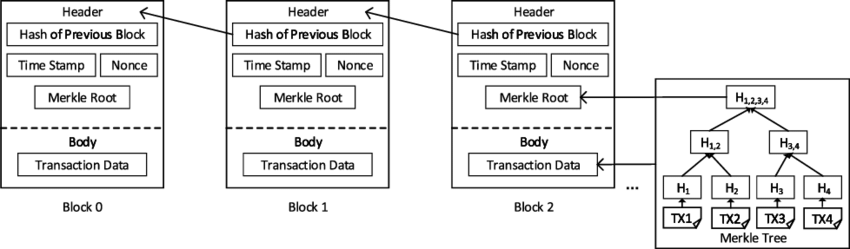
\includegraphics[scale=0.3]{images/block-blockchain.png}
        \caption{Blocos da BlockChain \cite{2}}
        \label{fig:Blocos da BlockChain}
    \end{figure}

    O \textit{header} consiste na hash do \textit{header} do bloco anterior, \textit{timestamp}, no \textit{nonce}, hash da \textit{data} e raiz da \textit{Merkle tree}, que representa todas as transações contidas no bloco.

    A \textit{Merkle tree} é uma estrutura de dados que agrupa as transações em pares, calcula a hash desses pares e, em seguida, repete o processo até que haja apenas uma hash no topo da árvore, que é a raiz. Essa raiz permite que os nós verifiquem rapidamente se uma transação específica está incluída no bloco sem a necessidade de processar todas as transações individualmente.
    Esta também contribui para a segurança da blockchain, uma vez que qualquer alteração numa transação resultaria numa mudança nas hashes, afetando a raiz de Merkle. Ou seja, é extremamente difícil manipular ou falsificar transações passadas, pois exigiria a modificação de todas as hashes subsequentes na árvore.

    A \textit{data} consiste na lista de transações e outras informações relevantes.
    Cada bloco é conectado ao bloco anterior por meio da função de hash no header, formando uma cadeia contínua de blocos. Essa estrutura garante a integridade dos dados, uma vez que qualquer alteração num bloco afetaria todos os blocos subsequentes.

    A blockchain suporta \textit{smart contracts}, que são projetados para automatizar, facilitar e fazer cumprir a execução de acordos e contratos entre as partes envolvidas, sem a necessidade de intermediários. Estes critérios são primeiro verificados na parte da aplicação tendo em conta a forma como o leilão funciona, ou seja, cada licitação é superior à anterior mais o incremento establecido pelo vendedor; para um participante fazer uma licitação tem de fazer a transferência do valor para o vendedor; e cada transação tem uma taxa associada para pagar ao minerador (esta recompensa é feita automaticamente quando a hash criada é verificada e cumpre os requisitos). No entanto, para criar o novo bloco, a blockchain verifica novamente se as transações que vão ser guardados naquele bloco estão em concordância com os requisitos.

    \subsection{Nodes}
    Assim na blockchain existem diferentes tipos de nós que interagem com a rede e desempenham funções específicas, embora apenas nos tenhamos focado em implementar os full nodes (\textit{BlockchainNodeType::Boostrap}) e os miner  nodes(\textit{BlockchainNodeType::Miner}). Podemos verificar como se organizam os diferentes tipos de nós na figura \cite{3} e como eles se relacionam na figura \cite{4}.

    \begin{figure}[H]
        \centering
        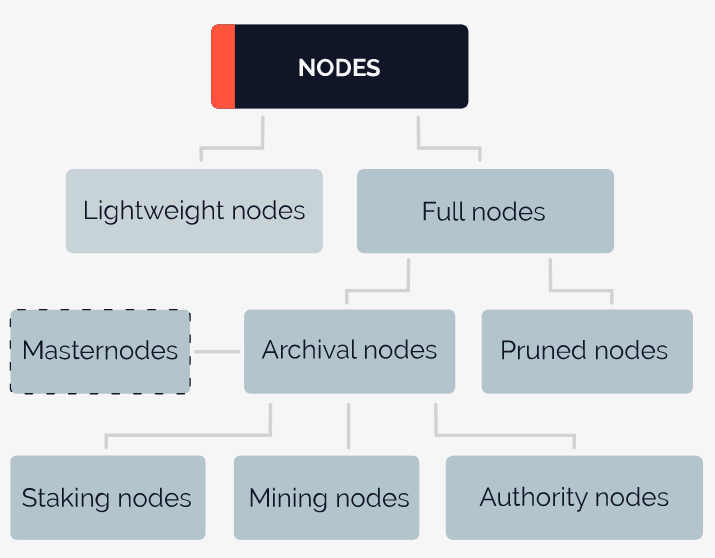
\includegraphics[scale=0.25]{images/types-of-nodes.png}
        \caption{Tipos de Nós \cite{3}}
        \label{fig:Tipos de Nós}
    \end{figure}
    \begin{figure}[H]
        \centering
        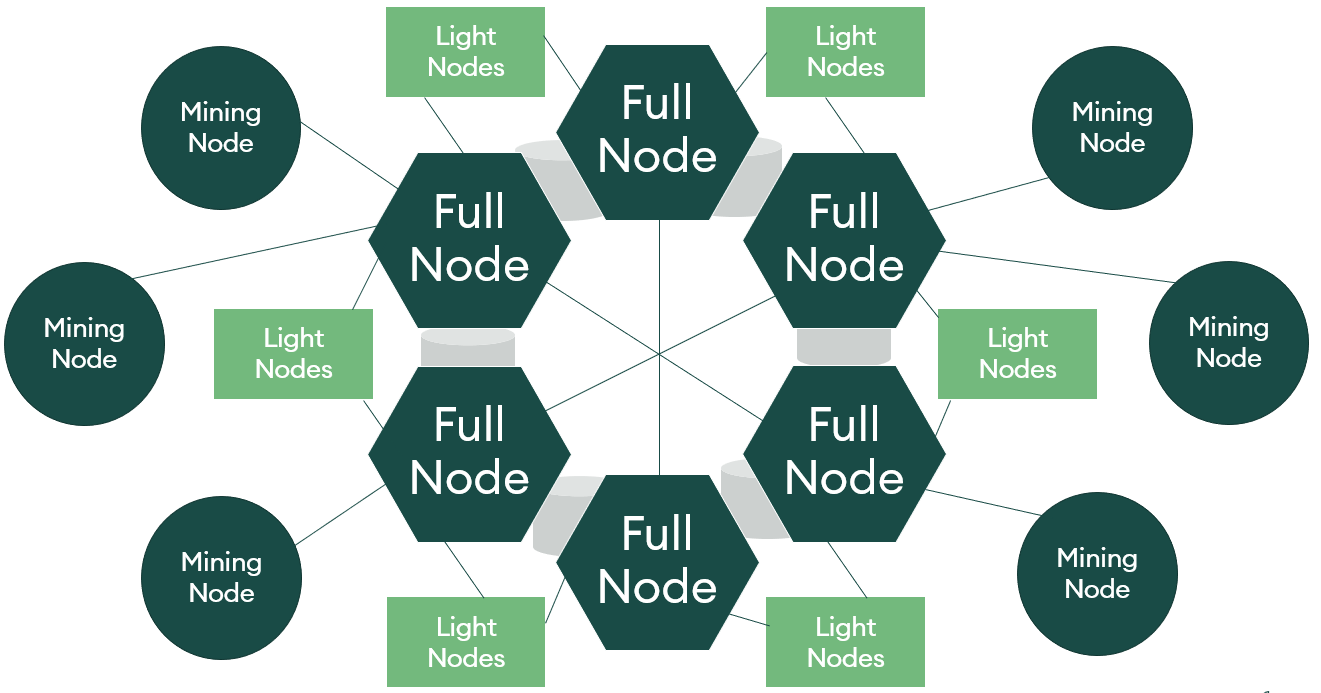
\includegraphics[scale=0.2]{images/nodes-interacting.png}
        \caption{Interação entre os Nós \cite{4}}
        \label{fig:Interação entre os Nós}
    \end{figure}


    Assim, os nós podem ser:
    \begin{itemize}
        \item \textbf{Light Nodes:} Nós que não armazenam uma cópia completa da blockchain, logo dependem de outros nós para obter informações sobre transações e blocos relevantes. Embora estes nós não tenham acesso a todos os detalhes da blockchain, podem verificar a autenticidade das transações e realizar operações básicas na rede.
        \item \textbf{Full Nodes:} Nós que mantêm uma cópia completa da blockchain na sua totalidade. Validam e verificam todas as transações e blocos, armazenando uma cópia atualizada do registo distribuído. Podem participar no processo de consenso, armazenar e propagar transações e blocos, e fornecer acesso a informações completas da blockchain para outros nós.
        \begin{itemize}
            \item \textbf{Pruned Nodes:} Armazenam apenas uma parte da blockchain, removendo dados antigos e não essenciais. Essa abordagem ajuda a reduzir o tamanho do armazenamento necessário para executar um nó completo. No entanto, os nós podados ainda podem verificar e validar transações recentes, mas não têm acesso a informações sobre transações mais antigas.
            \item \textbf{Archive Nodes:} Armazenam uma cópia completa e histórica de todos os blocos e transações da blockchain, permitindo a consulta e análise de transações antigas. Os nós de arquivo podem ser úteis para fins de auditoria, pesquisa ou análise de longo prazo da blockchain.
            \begin{itemize}
                \item \textbf{Masternodes:} Possuem funções adicionais de administração, serviços ou recursos avançados. Exigem uma quantidade mínima de tokens da blockchain como garantia para serem elegíveis como masternodes. Os masternodes podem desempenhar funções como facilitar transações instantâneas, votar em propostas de melhoria da rede ou fornecer serviços específicos para a blockchain.
                \item \textbf{Staking Nodes:} Participam no mecanismo de consenso Proof of Stake. Neste mecanismo, os nós "apostam" os seus tokens como garantia para validar transações e criar novos blocos. Os nós de stake são selecionados para criar blocos com base na quantidade de tokens que estão apostados. Estes são recompensados com mais tokens, como incentivo por a sua participação no consenso.
                \item \textbf{Mining Nodes:} Responsáveis por adicionar novos blocos à blockchain por meio do processo de mineração. Os nós de mineração competem entre si para resolver problemas matemáticos complexos, de modo a encontrar um novo bloco válido. Quando um nó de mineração encontra a solução correta, adiciona o novo bloco à blockchain e é recompensado com as taxas de transação.
                \item \textbf{Authority Nodes:} Têm autoridade para validar transações e fazer decisões sobre a administração da blockchain. São selecionados com base em regras específicas e desempenham um papel importante na segurança e consenso da rede.
            \end{itemize}
        \end{itemize}
    \end{itemize}

    \subsection{Proof of Work}
    Além disso, a blockchain utiliza um mecanismo de consenso, como o Proof of Work (PoW), para garantir que todos os nós da rede concordem na validade das transações e a ordem em que são adicionadas aos blocos.

    Na Proof-of-Work, os mining nodes devem provar que realizaram um trabalho computacional difícil antes que os seus blocos sejam aceites pela rede. Esse trabalho computacional envolve a resolução de um problema matemático complexo, uma função de hash criptográfica.

    Assim, para isto o mining node recebe um conjunto de transações que deseja adicionar a um novo bloco e combina essas transações com um valor aleatório chamado "nonce" (número usado apenas uma vez) e calcula o hash do bloco resultante.
    O hash do bloco deve atender a determinados critérios para ser considerado válido. Neste caso, os critérios exigem que o hash comece com 10 zeros, o que torna o cálculo do hash difícil e requer tentativa e erro.

    Assim este nó itera o hash varias vezes com diferentes valores de nonce até encontrar um que resulte num hash válido. Isso requer poder computacional significativo e consome tempo.

    Uma vez que o mining node encontre um nonce válido antes de outros mining nodes encontrarem, adiciona o bloco à cadeia e o propaga para a rede que encontrou e o que encontrou. Os outros participantes da rede verificam se o hash do bloco é válido, executando a mesma função de hash e verificando se os critérios são atendidos.

    Se o hash for válido, o bloco é aceite e adicionado à blockchain. O minerador que encontrou o nonce válido é recompensado, incentivando a participação dos mineradores no processo.

    Assim, é criado um sistema em que é necessário um esforço computacional significativo para criar novos blocos, o que dificulta a adulteração da cadeia de blocos por parte de participantes mal-intencionados. Além disso, como a solução do problema requer poder computacional, a adição de novos blocos é um processo relativamente lento, impedindo a criação de blocos falsos em rápida sucessão.

    \subsection{Outros mecanismos de consenso}
    Como o registro distribuído é modular, permite assim a adição de novos mecanismos de consenso, como Proof-of-Stake (PoS) ou BFT.
    \subsubsection{Proof-of-Stake}
    A Proof-of-Stake é um algoritmo de consenso utilizado para validar transações e criar novos blocos. Ao contrário do Proof-of-Work, que requer que os participantes resolvam problemas computacionais complexos para validar transações, o Proof-of-Stake atribui o direito de criar um novo bloco com base na participação de criptomoedas que o participante possui e está disposto a "apostar" como garantia.

    Neste caso, os nós participantes da rede que desejam atuar como validadores (também conhecidos como stakers) devem demonstrar a posse de uma quantidade mínima de tokens da criptomoeda nativa da blockchain, ainda não definida.
    O algoritmo de seleção do validador pode ser baseado em diferentes critérios, como a quantidade de tokens apostados, a antiguidade dos tokens ou um sistema de votação entre os nós. Isso determinará qual nó será responsável por criar o próximo bloco.
    O validador selecionado cria um novo bloco, verifica as transações e assina digitalmente o bloco utilizando sua chave privada. A quantidade de tokens apostados pelo validador influencia a sua probabilidade de ser selecionado para criar o bloco.
    Os restantes nós da rede validam o bloco criado pelo validador, verificando a assinatura digital e a integridade das transações. Eles verificam também se o validador cumpriu as regras estabelecidas pelo protocolo.
    Os validadores selecionados para criar novos blocos recebem recompensas na forma de novas unidades da criptomoeda. No entanto, se um validador for detectado a realizar atividades maliciosas ou a não cumprir regras, ele é penalizado e fica com parte ou todos os seus tokens confiscados.
    A aplicação de Proof-of-Stake neste projeto permitiria uma maior eficiência energética em comparação ao Proof-of-Work, pois não exigiria um consumo computacional intensivo. Além disso, o Proof-of-Stake incentiva a participação ativa dos detentores de tokens na rede, uma vez que eles têm a oportunidade de serem selecionados como validadores e receberem recompensas proporcionais à sua participação. No entanto, ao contrário da Proof-of-Work este consenso é mais suscetivel a ataques de segurança.

    \subsubsection{BFT (Byzantine Fault Tolerance)}
    Byzantine Fault Tolerance é um conceito na área de sistemas distribuídos que visa alcançar um consenso confiável entre os participantes, mesmo quando ocorrem falhas ou comportamentos maliciosos de nós na rede.

    Assim para aplicar este mecanismo, em vez de confiar num único nó para replicar e manter os dados da blockchain, o sistema pode adotar uma abordagem de replicação, onde várias cópias dos dados são mantidas em nós diferentes. Essa replicação distribuída aumenta a resistência a falhas e ataques maliciosos.
    Este algoritmo de consenso Bizantino permite que os nós na rede cheguem a um acordo na validade das transações e na ordem na qual elas devem ser adicionadas à blockchain. O objetivo é garantir que mesmo que alguns nós sejam comprometidos ou ajam de maneira maliciosa, o consenso geral ainda possa ser alcançado entre os nós honestos.
    O BFT requer que os nós se comuniquem entre si de maneira segura e confiável, mesmo num ambiente adversário, ou seja, utilizando criptografia de chave pública. Assim, o objetivo principal do BFT é permitir que o sistema continue a operar corretamente, mesmo quando alguns nós apresentam falhas ou se comportam de maneira maliciosa. Os algoritmos BFT são projetados para resistir a uma certa percentagem de nós maliciosos na rede.\\


    \section{Mecanismos de leilão (\textit{Auction mechanisms})}

    Os mecanismos de leilão utilizados são baseados no modelo de leilão inglês, utilizando um atributo único para cada leilão.
    Assim sendo, o vendedor deve iniciar o leilão com um preço inicial definido por ele e ainda definir o valor do incremento para cada licitação. Desta forma, cada licitação deve ser superior ao valor anterior licitado. Assim, o leilão deve ser aberto, ou seja, todos os participantes podem ver as licitações anteriores feitas pelos concorrentes e assim basearem-se nisso para fazerem a sua oferta. O vencedor do leilão é determinado pela última oferta antes de encerrar o leilão e o participante que a fez é obrigado a pagar o seu valor para obter o produto leiloado.
    Os leilões são suportados por um sistema de publicador/assinante, que mantém registo dos participantes de cada leilão e assim informa os utilizadores de cada transação, para que possam acompanhar as informações sobre os leilões em tempo real. Todas transações de leilão e licitações são guardadas na blockchain, sendo que a informação é guardada em blocos, logo várias transações são guardadas no mesmo bloco, permitindo uma maior transparência, segurança e eficiência no processo.

    De forma a evitar especulação por parte dos licitadores, decidimos que para fazer uma licitação os utilizadores devem fazer a transferência do valor monetário para o vendedor e se o vendedor aceitar fica fechado o leilão e tem-se um novo resultado, caso ele rejeite, o leilão continua. Assim, é do interesse do vendedor não aceitar o pagamento, para que venda o produto o mais caro possivel. De forma a gerir as recompensas dos mineradores, para um utilizador fazer uma transação, este terá que pagar uma taxa, sendo esta a recompensa dos mineradores.

    Para além disto, esta aplicação utiliza criptografia de chave publica, de modo a conferir confidencialidade e integridade em cada operação. Cada participante da rede tem um par de chaves criptográficas, privada e pública. A chave pública é partilhada com outros participantes, enquanto a chave privada é mantida em segredo. Ao comunicar com os outros participantes, a chave pública é usada para verificar a identidade do remetente, garantindo que a comunicação seja autêntica. Ao realizar transações ou publicar informações na blockchain, um participante assina digitalmente esses dados para garantir que são autênticos e que não foram alterados. Os outros participantes podem verificar a assinatura usando a chave pública do remetente para confirmar a autenticidade dos dados.\\


    \section{Conclusão}
    Concluindo, neste projeto, ao integrar o protocolo \textit{Kademlia DHT} para fazer a rede distribuída que gere os utilizadores e produtos, e a blockchain para armazenar toda a informação sobre transações (licitações e leilões) criamos uma aplicação que garante a segurança e transparência de um sistema de leilões, no modelo inglês. Esta segurança é dada pelos mecanismos utilizados, nomeadamente, o grau de confiança de um nó, a Proof-of Work, e ainda temos a possibilidade de implementar a Proof-of-Stake ou a BFT, que ao contrário da Proof-of-Work torna o sistema mais rápido e eficiente, no entanto, oferece uma menor segurança.
    Por fim, a aplicação é capaz suportar compradores e vendedores, e verifica todos os requisitos para o funcionamento correto de um leilão, e também mantém o registo de todas as transações, para consultas futuras.\\


    \begin{thebibliography}{1}
        \bibitem{1} D. P. Acharya, “An In-Depth Guide on the Types of Blockchain Nodes,” Geekflare, Dec. 2022, [Online]. Available: \href{https://geekflare.com/blockchain-nodes-guide/}{here}.
        \bibitem{2} “A importancia de rodar um nó (node)?,” TriboCrypto, Dec. 26, 2019, [Online]. Available: \href{https://tribocrypto.com/t/a-importancia-de-rodar-um-no-node/830}{here}.
        \bibitem{3} J. Frankenfield, “What Is Proof of Work (PoW) in Blockchain?,” Investopedia, Feb. 2023, [Online]. Available: \href{https://www.investopedia.com/terms/p/proof-work.asp}{here}.
        \bibitem{4} J. Frankenfield, “What Does Proof-of-Stake (PoS) Mean in Crypto?,” Investopedia, Apr. 2023, [Online]. Available: \href{https://www.investopedia.com/terms/p/proof-stake-pos.asp}{here}.
        \bibitem{5} “Distributed Hash Tables with Kademlia — Stanford Code the Change Guides  documentation.” \href{https://codethechange.stanford.edu/guides/guide\_kademlia.html}{here}.
        \bibitem{6} GeekLaunch, “Adding Transactions to the Blockchain: Concepts - Blockchain in Rust \#04: Transactions 1,” YouTube. Feb. 06, 2019. [Online]. Available: \href{https://www.youtube.com/watch?v=-k1Yk9D\_lU4}{here}.
        \bibitem{7} J. Fáwolé, “Sybil Attack in Blockchain: Examples \& Prevention,” Hacken, Apr. 2023, [Online]. Available: \href{https://hacken.io/insights/sybil-attacks/}{here}.
        \bibitem{8} Satoshi Nakamoto. Bitcoin: A peer-to-peer electronic cash system. 2008.
        \bibitem{9} Ingmar Baumgart and Sebastian Mies. S/kademlia: A practicable approach towards secure key-based routing. In Parallel and Distributed Systems. 2007.
    \end{thebibliography}
\end{document}


